Integer programming expands upon the possible problems that can be modeled by
linear programming. Whereas decision variables in linear programming are
optimized on a continuum, i.e., all decision variables are real numbers,
$x \in \mathbb{R}^n$. Integer programming allows for decision variables to take
on integer-only values, i.e., $y \in \mathbb{Z}^n$. Strictly speaking, a
programming formulation for which all decision variables are integer (i.e.,
integer and binary) is called an \textit{integer program} (IP), whereas a
programming formulation for which some deicision variables are integer while
others are linear is called a \textit{mixed integer-linear program} (MILP). The
discussion that follows is informed largely by Wolsey's
text \cite{wolsey_integer_1998} from which I cite many definitions,
etc. Additional clarification comes from class notes \cite{luedtke_class_2010}.

Integer programming allows one to model specialized decision cases. Take for
example one of the most well-known problems in mathematical programming and
optimization, the \textit{Knapsack Problem}. The Knapsack problems is described
as follows:

\begin{itemize}
        \item A knapsack can hold at most $b$ pounds. 
        \item There are $n$ possible items that can be placed in the bag.
        \item Each item is characterized by a preference, or benefit, $c_i$, 
              and a weight, $a_i$
        \item One would like to maximize the benefit associated with a knapsack
\end{itemize}

The decision variables, $y_i$s, for the Knapsack Problem provide its integer
nature. Any given item in the above formulation can only be added once. Indeed,
consider that for any viable solution, each item is in one of two distinct
states: included in the knapsack or excluded from the knapsack. This duality of
states provides a natural usage of binary variables, i.e., a variable that has
only two states, 0 and 1. Accordingly, the Knapsack Problem as an integer
program is formulated as Equation \ref{eqs:knapsack}.

%%% 
\begin{subequations}\label{eqs:knapsack}
  \begin{align}
    %%
    \max \:\: & 
    \sum_{i \in I} c_i y_i
    & \\
    %%
    \text{s.t.} \:\: &
    \sum_{i \in I} a_i y_i \leq b 
    & \\
    %%
    &
    y_i \in \{ 0, 1 \}
    &
    \forall i \in I
    %%
  \end{align}
\end{subequations}
%%% 

\subsection{Computational Complexity}\label{sec:complexity}

In general, optimization problems are solved by solving a number of decision
problems. Decision problems are generally
computationally \textit{hard}. Decision problems ask yes or no questions,
e.g. ``is there a knapsack packing that with a benefit higher than $x$?''. An
optimization problem asks instead ``what is the knapsack packing with the
highest benefit?''. Any problem can be associated with one of four categories of
computational complexity:

\begin{itemize}
        \item Polynomial ($\mathcal{P}$)
        \item Nondeterministic Polynomial ($\mathcal{NP}$)
        \item Nondeterministic Polynomial Complete  ($\mathcal{NP}$-C)
        \item Nondeterministic Polynomial Hard  ($\mathcal{NP}$-hard)
\end{itemize}

The topic of computational complexity is relatively involved, thus I will only
provide a short overview to simply provide context. A problem is considered to
reside in $\mathcal{P}$ if there is a polynomial-time algorithm that can solve
it. A classic example is that of naive matrix inversion, known to be of order
$n^3$ (i.e., $\mathcal{O}(n^3)$) for a given $n$ x $n$ matrix.

A decision problem is considered to be in ($\mathcal{NP}$) if for any proposed
solution, there is a \textit{short certificate}.

\begin{define}
A \textbf{certificate} is a method to verify that a solutions provides a
positive or negative response to the question at hand. A certificate is
considered \textbf{short} if it is polynomial in size and can be verified in
polynomial time.
\end{define}

A decision problem, $Q$, is considered to be in $\mathcal{NP}$-C, if
$Q \in \mathcal{NP}$ and \textit{any} problem, $P \in \mathcal{NP}$ is
polynomially reducable to $Q$, i.e., instances of $P$ can be reformulated as
instances of $Q$ in polynomial time. The most popular candidate of this
polynomial reduction is the Satisfiabiliy Problem, known to be in
$\mathcal{NP}$-C.

Finally, a problem $Q$, is in $\mathcal{NP}$-hard, if any problem
$P \in \mathcal{NP}$ is polynomially reducible to $Q$, but
$Q \not\in \mathcal{NP}$. If a decision problem is in $\mathcal{NP}$-C, then the
corresponding optimization problem is $\mathcal{NP}$-hard.

The various levels of complexity are related. It is not known whether
$\mathcal{P} = \mathcal{NP}$, but it is strongly suspected that
$\mathcal{P} \subset \mathcal{NP}$. Of course
$\mathcal{NP}\text{-C} \subset \mathcal{NP}$, and
$\mathcal{NP}\text{-hard} \notin \mathcal{NP}$ by definition. The relationship
between these set of problem complexities is shown graphically in
Figure \ref{fig:complexity}.

\begin{figure}[H]
  \begin{center}
    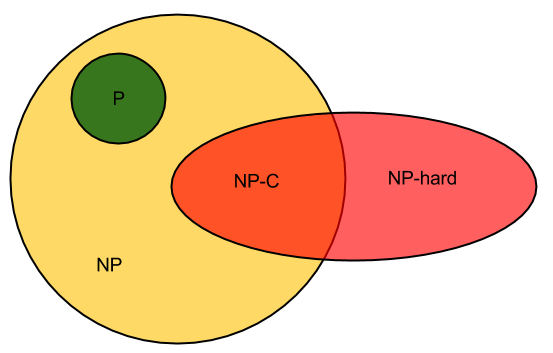
\includegraphics[width=\linewidth]{./chapters/litreview/complexity.png}
  \caption{The relationship between the various types of problem complexities.}
  \label{fig:complexity}
  \end{center}
\end{figure}


\subsection{Formulations and Cutting Planes}\label{sec:formulations}

Optimization problems are given as formulations, a series of inequality
equations. Both domain knowledge and geometrical investigation can provide
better formulations than may be evident from an initial formulation. Formally, a
formulation forms a polyhedron.

\begin{define}\label{def:polyhedron}
A subset of $\mathbb{R}^n$ described by a finite set of linear constraints $P
= \{ x \in \mathbb{R}^n : Ax \leq b\}$ is a \textbf{polyhedron}.
\end{define}

\begin{define}\label{def:formulation}
A polyhedron $P \subseteq \mathbb{R}^{n+p}$ is a \textbf{formulation} for a set
$X \subseteq \mathbb{Z}^n \times \mathbb{R}^p$ iff $X = P \cap \left( 
\mathbb{Z}^n \times \mathbb{R}^p \right)$
\end{define}

As previously noted, more than one formulation can be viable for a given
problem. Let us return to the Knapsack Problem in
Equation \ref{eqs:knapsack}. Consider a knapsack with $b = 5$ and items with
$a_1 = 2$, $a_2 = 3$, $a_3 = 4$. The original formulation is as follows.

%%% 
\begin{subequations}\label{eqs:knapsack1}
  \begin{align}
    %%
    \max \:\: & 
    \sum_{i \in I} c_i y_i
    & \\
    %%
    \text{s.t.} \:\: &
    2y_1 + 3y_2 + 4y_3 \leq 5 
    & \\
    %%
    &
    y_i \in \{ 0, 1 \}
    &
    \forall i \in I
    %%
  \end{align}
\end{subequations}
%%% 

The set of feasible solutions here forms a polyhedron from the points $Y = {(0,
0, 0), (1, 0, 0), (0, 1, 0), (0, 0, 1), (1, 1, 0)}$. The optimal solution will
depend on values given to each item's benefit, $c_i$. However, the formulation
as provided defines a solution space larger than the specific points mentioned
here. One could add a constraint, say, 

\begin{equation*}
y_1 + y_3 \leq 1
\end{equation*}

or 

\begin{equation*}
y_2 + y_3 \leq 1.
\end{equation*}

These two constraints state that the third item, if chosen, can not be included
with either the first or the second item. The resulting formulation is shown in
Equation \ref{eqs:knapsack2}.

%%% 
\begin{subequations}\label{eqs:knapsack2}
  \begin{align}
    %%
    \max \:\: & 
    \sum_{i \in I} c_i y_i
    & \\
    %%
    \text{s.t.} \:\: &
    2y_1 + 3y_2 + 4y_3 \leq 5 
    & \\
    %%
    &
    y_1 + y_3 \leq 1        
    & \\
    %%
    &
    y_2 + y_3 \leq 1        
    & \\
    %%
    &
    y_i \in \{ 0, 1 \}
    &
    \forall i \in I
    %%
  \end{align}
\end{subequations}
%%% 

It is obvious that Equation \ref{eqs:knapsack2} is a different formulation than
Equation \ref{eqs:knapsack1}. For example, the point $(0.9, 0.5, 0.4)$ resides
in the feasible solution space of Equation \ref{eqs:knapsack1} but is outside of
the feasible solution space of Equation \ref{eqs:knapsack2}. Intuitively, a
smaller solution space can be searched more quickly, thus \textit{tighter}
formulations require less time to solve in general.

The notion of one formulation being ``better'' than another can be formally
expressed.

\begin{define}
Given a set $X \subseteq \mathbb{R}^n$ and two formulations, $P_1$ and $P_2$,
for $X$, $P_1$ is a \textbf{better formulation} than $P_2$ if $P_1 \subset P_2$.
\end{define}

There is, of course, a limit to the formulations one can develop for a given
problem. A fully-restricted solution space, i.e., one that is as tightly bounded
as possible, is called the problem's \textit{convex hull}. 

\begin{define}
Given a set $X \subseteq \mathbb{R}^n$, the \textbf{convex hull} of $X$, denoted
$conv(X)$, is defined as: $conv(X) = \{x : x = \sum_{i=1}^{t} \lambda_i
x_i, \sum_{i=1}^{t} \lambda_i = 1, \lambda_i \geq 0$ for $i = 1, \ldots, t$ over
all finite subsets $\{x^1, \ldots, x^t \}$ of $X\}$.
\end{define}

Because the extreme points of $conv(X)$ all lie in $X$, the equivalent LP can be
used instead of the IP. Convex hull formulations are rarely seen in practice,
however, because they require an exponential number of additional
constraints \cite{wolsey_integer_1998}. While the convex hull of a given problem
may not be discovered in practice, the feasible solution space most assuredly is
reduced by most solution techniques. From a geometrical point of view, this acts
as cutting off solution space from some original larger space through the
addition of constraints as shown above. Accordingly, these constraints are
termed \textit{cutting planes}.

\subsection{The Branch and Bound Algorithm}\label{sec:bnb}
\input{./chapters/litreview/bnb}
